\section{Diamond-Square}
\subsection{Sequential algorithm}
Fractal terrain generation can be achieved using the Diamond-Square algorithm introduced by Fournier, Fussel, Carpenter\cite{fournier1982computer} and Miller\cite{miller1986definition}. This algorithm computes a high resolution terrain through multiple iterations, each containing a \textit{square} and \textit{diamond} pass.

The final resolution is as follows:

\begin{equation}
(width_K, height_K) = 2^{K} ((width_0, height_0) - 1) + 1
\end{equation}

With \textit{L} the terrain width or height and \textit{K} the number of iterations. Therefore, each iteration increases the resolution according to $L_{k+1} = 2 L_k - 1$.

Note that if we don't use an initial terrain, $2^K = L$.

\begin{figure}[!htb]
\minipage{0.5\textwidth}
    \centering
    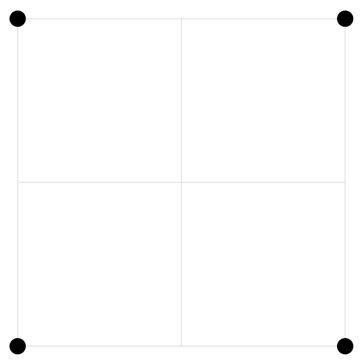
\includegraphics{img/ds_init.jpg}
    \caption{Initial matrix}
\endminipage\hfill
\minipage{0.5\textwidth}
    \centering
    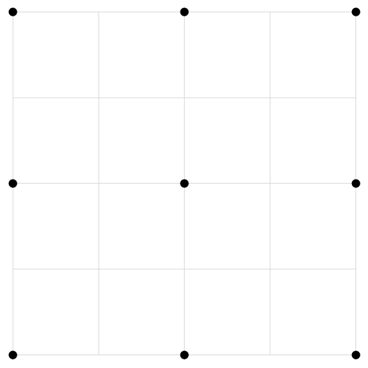
\includegraphics{img/ds_final.jpg}
    \caption{Matrix after the first iteration}
\endminipage\hfill
\end{figure}

To reduce the computation time, we have optimized the memory management by removing the memory allocation and release required by the change of matrix dimensions. Hence, we use a single matrix which has the final terrain dimension. This matrix is actually a simple height map. However, to simplify the algorithm, each iteration only consider a \textit{virtual} matrix which is a part of the final matrix. This matrix has the size expected at the end of the iteration, and we use the following formula to switch from virtual to real matrix coordinates:

\begin{equation}
(i_K, j_K) = 2^{K - k} (i_k, j_k)
\end{equation}

\subsubsection{Randomness}
In order to make our terrain less smooth and thereforemore more realistic, we add a random factor when computing the new points of our terrain.

The random factor \textit{r} is generated according to $0 \leq r \leq scale_k$, with $scale_{k+1} = \frac{scale_k}{2}$.


\subsubsection{Square pass}
The square pass aims at computing the value located at the center of a \textit{square}. This value is the average of those four points.

\begin{equation}
m(i, j) = \frac{m(i-1, j-1) + m(i-1, j+1) + m(i+1, j-1) + m(i+1, j+1) + r)}{4}
\end{equation}

\begin{figure}[H]
\centering
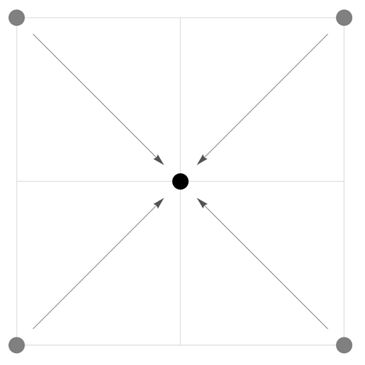
\includegraphics[width=0.3\textwidth]{img/ds_square.jpg}
\caption{Square pass}
\end{figure}

\subsubsection{Diamond pass}
In a similar way, the diamond pass computes the average of four other points as described in figure \ref{fig:ds_diamond}.

\begin{equation}
m(i, j) = \frac{m(i-1, j) + m(i+1, j) + m(i, j-1) + m(i, j+1) + r)}{4}
\end{equation}

\begin{figure}[H]
\centering
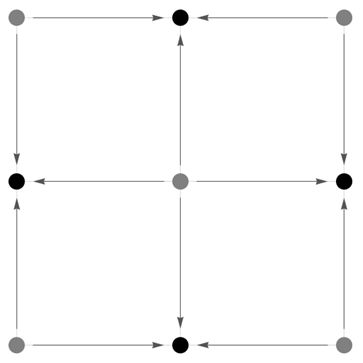
\includegraphics[width=0.3\textwidth]{img/ds_diamond.jpg}
\caption{Diamond pass}
\label{fig:ds_diamond}
\end{figure}


\subsubsection{Water level}
Optionally, every value in the height map below a certain thresold can be set to this threshold after the \textit{K} iterations. This operation can be considered as pouring water on the terrain to give a more realistic rendering.


\subsection{Parallelization}
\subsubsection{Processes topology}
In order to make our program more user friendly, this one takes as input the number of processes \textit{N} and computes the best processes topology $P Q$. This is achieved by computing the two highest factors such that $N = P Q$.

A process coordinates $(p, q)$ in the processes topology is therefore
\begin{equation}
\begin{split}
p = rank \mod P\\
q = \frac{rank}{P}
\end{split}
\end{equation}

While its rank is $rank = q  P + p$

\subsubsection{Scatter and gather data}
Since $P_0$ is the only process importing and exporting the terrain, this algorithm obviously contain a \textit{scatter} (one-to-all) and \textit{gather} (all-to-one) phase, while data is exchanged between $P_0$ and the other processes. To reduce the amount of data exchanged and the memory consumption, each process (except $P_0$) knows only the part of the terrain which has been assigned to it.

The matrix dimensions of a process given its coordinates in the processes grid is given below, with \textit{N} the number of processes ($\sqrt{N}$ is P if we distribute the data width, Q otherwise). This formula guarantees the best linear data distribution on each axis. For simplification, we use $L = length = width = height$

\begin{equation}
\label{eq:ds_data_complexity}
L = \frac{L + \sqrt{N} - 1}{\sqrt{N}} + 
\mathbbm{1}_{rank < (L + \sqrt{N} - 1) \mod \sqrt{N}}
\end{equation}

\subsubsection{Parallel Diamond-Square}
The Diamond-Square algorithm computed by each process is almost the same as previously described. However, we can observe that the diamond pass requires data from other processes. Since each point located at the border of the matrix must be computed based on the values computed by the square pass of two different processes, those \textit{ghost cells} must be exchanged at the end of each iteration using a two-dimensions red-black communication.

The data exchanged only contain $\frac{L_k - 1}{2}$ data points, i.e. the output of the previous square pass for the corresponding terrain side.

\begin{figure}[H]
\centering
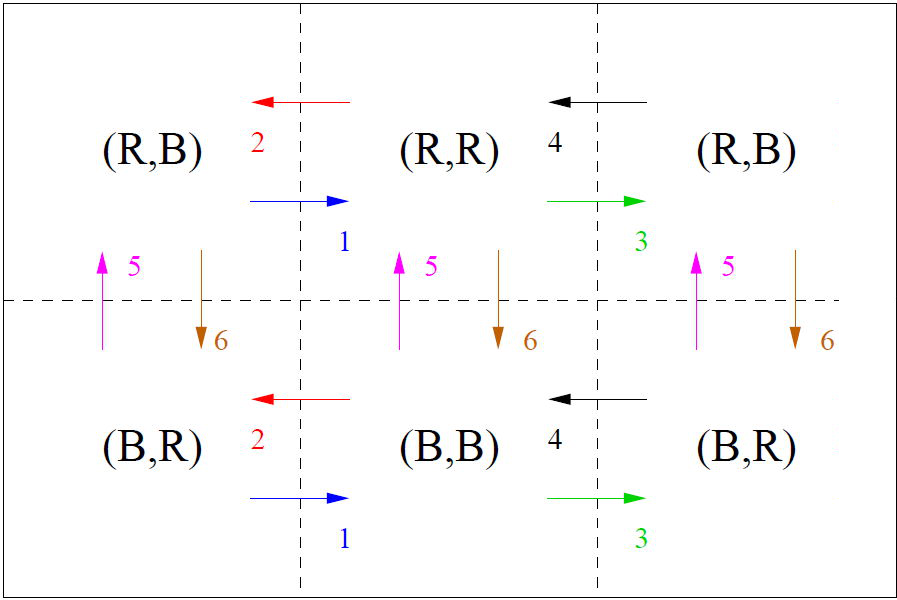
\includegraphics[width=0.6\textwidth]{img/ds_red_black.png}
\caption{Red-Black communication algorithm}
\end{figure}

Since the diamond pass computation also includes a random factor, this one is added to the ghost cells sent by a left-rigth or up-down communication so that each process work with the same data.

After this communication step, the diamond pass is finalized by computing the data points on the four sides of the height map.


\subsubsection{Parallel algorithm}
The parallelized algorithm is eventualy
\begin{lstlisting}
initMPI(argc, argv, &N, &rank);

// Computes the process topology and return the process coordinates
getProcessTopology(N, &P, &Q, &p, &q); 

// Read the initial matrix from an input file then send to each process the part it has to compute
data = importAndScatterData(rank, inputFile, &height, &width, &initWidth, &initHeight, iterations, P, Q);

// Diamond-Square algorithm, including data exchange
diamondSquare(data, initWidth, initHeight, iterations, p, q, P, Q);

// Pour water on the terrain so that every point below the water level is raised to this level
pourWater(data, height, width);

// Gather final data from every process then complete the data matrix for final result
gatherData(data, height, width, rank, P, Q, iterations);

if(rank == 0) {
    // Export the final terrain in the output file
    exportData(data, FINAL_TERRAIN_HEIGHT, FINAL_TERRAIN_WIDTH, outputFile);
}

// Release memory and finalizes MPI
clear(data, height);
\end{lstlisting}

\begin{figure}[!htb]
\minipage{0.5\textwidth}
    \centering
    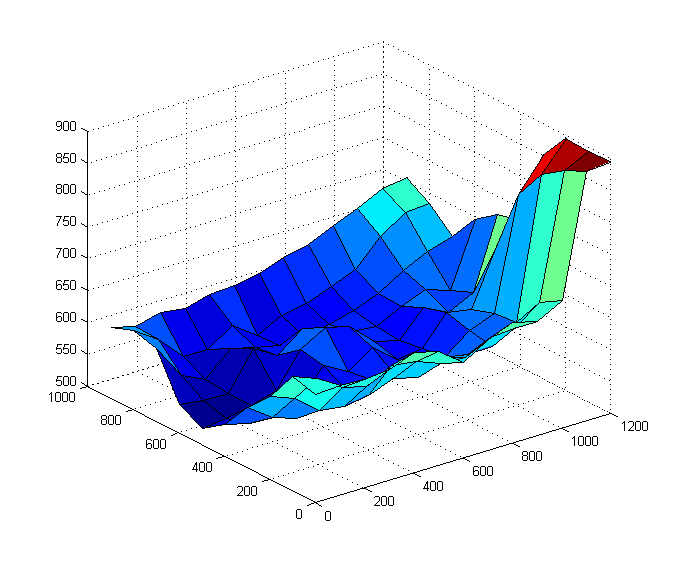
\includegraphics[width=\linewidth]{img/init.png}
    \caption{Initial terrain (13x10)}
\endminipage\hfill
\minipage{0.5\textwidth}
    \centering
    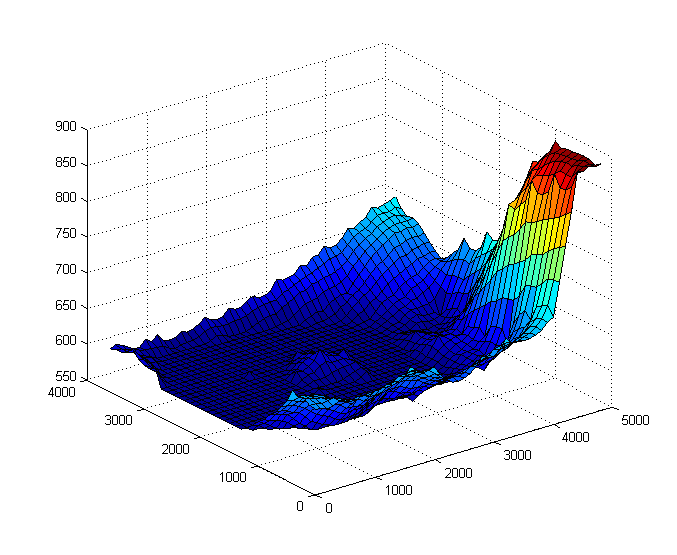
\includegraphics[width=\linewidth]{img/final.png}
    \caption{Final terrain - 2 iterations (49x37)}
\endminipage\hfill
\end{figure}

\subsection{Parallel efficiency}
\subsubsection{Complexity}
The complexity of the Diamond-Square algorithm is obtained as follows, assuming a perfectly load balanced linear data distribution, $\sqrt{N} = P = Q$
Seeing that  for the {\em Diamond-Square} step we have a complexity of

\begin{multline}
\underbrace{\order\left((N-1) \left(\frac{L_0 + N - 1}{\sqrt{N}}\right)^2\right)}_{\text{scatter data}} + \order\left(\sum\limits_{k = 1}^{K} \text{square} + \text{diamond} + \text{exchange} + \text{update diamonds}\right) +\\+ \underbrace{\order\left((N-1) \left(\frac{L_K}{\sqrt{N}}\right)^2\right)}_{\text{gather data}}
\end{multline}

$L_k$ is the data width or height at iteration k. Hence, $L_K^2$ is the final terrain dimension, with K the total number of iterations. The complexity for an iteration is

\be
\underbrace{
    \underbrace{\order\left(\left(\frac{L_k}{2\sqrt{N}}\right)^2 \right)}_{\text{square}} +
    \underbrace{\order\left(\frac{(L_k/\sqrt{N})^2}{2} \right)}_{\text{diamond}} + 
    \underbrace{\order\left(\frac{4 L_k}{2\sqrt{N}}\right)}_{\text{exchange}} + 
    \underbrace{\order\left(\frac{4 L_k}{2\sqrt{N}}\right)}_{\text{update diamonds}}
 }_{\text{Diamond-Square}}
\ee

We eventually get the total complexity
\begin{equation}
\begin{split}
\order\left(L_0^2 + \sum\limits_{k = 1}^{K} \left(\left(\frac{L_k}{\sqrt{N}}\right)^2 \, + \left(\frac{L_k}{\sqrt{N}}\right)^2 \, + \frac{L_k}{\sqrt{N}}\, + \frac{L_k}{\sqrt{N}}\right) + L_K^2\right)\\
= \order\left(L_0^2 + \sum\limits_{k = 1}^{K} \frac{L_k^2}{N}\right)\\
= \order\left(\frac{L^2}{N}\right)
\end{split}
\end{equation}

This last step is obtained by solving the geometric series for $L_K \approx 2^K$ when starting with an empty terrain.

Eq.~\ref{eq:ds_data_complexity} gives us the data distribution. Based on this equation, the distribution is almost optimal:
\be
\frac{L + \sqrt{N} - 1}{\sqrt{N}} + \mathbbm{1}_{rank < (L + \sqrt{N} - 1) \mod \sqrt{N}} \underset{L\to +\infty}{\longrightarrow} \frac{L}{\sqrt{N}}
\nonumber
\ee

\subsubsection{Benchmarks and speedup}
According to fig.~\ref{fig:benchmarks_ds}, we can observe that our algorithm scales quite poorly. If the computation of the terrain scales quite efficiently, the loss of performances is mostly caused by the important communication cost when gathering data. Indeed, fig.~ \ref{fig:benchmarks2_ds} shows a much more interesting speedup without data gathering.

\begin{figure}[!htb]
\minipage{0.5\textwidth}
    \centering
    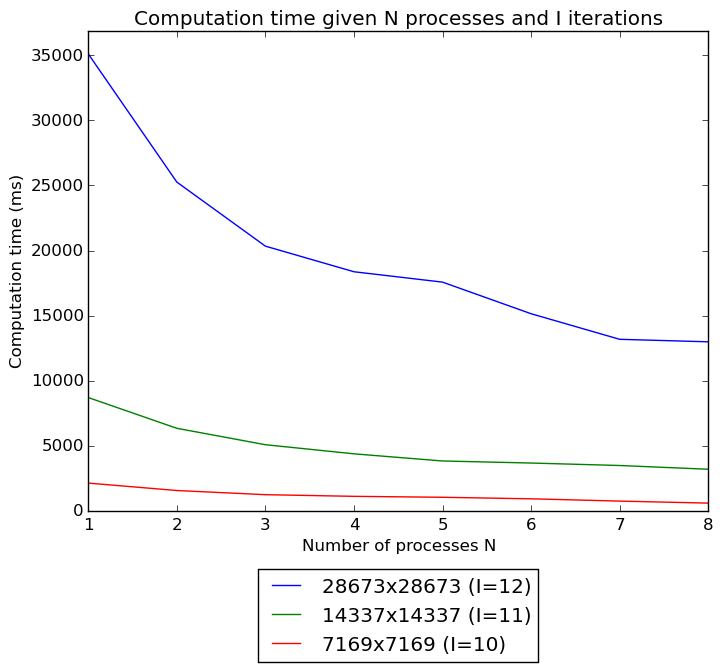
\includegraphics[width=\linewidth]{img/ds_benchmarks1.png}
    \caption{Benchmarks}
    \label{fig:benchmarks_ds}
\endminipage\hfill
\minipage{0.5\textwidth}
    \centering
    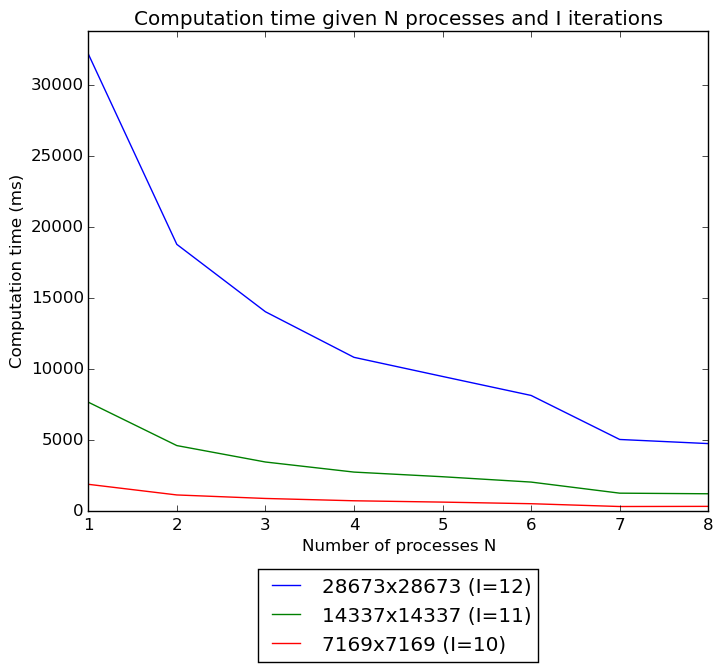
\includegraphics[width=\linewidth]{img/ds_benchmarks2.png}
    \caption{Benchmarks - No data gathering}
    \label{fig:benchmarks2_ds}
\endminipage\hfill
\end{figure}

\pagebreak

Because of the amound of data exchanged at the end of the algorithm, we obtain the speedups for an output resolution of 28673x28673 visible in table~\ref{table:speedup}. We assume $T^{\*}_s \approx T_1$ since our algorithm do not contain any communication or additional computation when $N = 1$.

\begin{table}[H]
\begin{center}
\begin{tabular}{c|c|c|c|c|}
 & \multicolumn{2}{c|}{Gathering} & \multicolumn{2}{c|}{Without Gathering} \\
\hline
Processes & $T_p$ [s] & $S_p$ & $T_p$ [s] & $S_p$ \\

\hline
$2$ & 25.256 & 1.39 & 18.773 & 1.71 \\
$4$ & 18.370 & 1.91 & 10.820 & 2.97\\
$8$ & 12.990 & 2.70 & 4.746 & 6.78\\
\hline
\end{tabular}
\caption{\label{table:speedup} Running time $T_p$ and speedup $S_p$ for different amount of processes. The running time for a single process is $T^{\*}_s = 35.100$~s with gathering and $T^{\*}_s = 32.186$~s without.}
\end{center}
\end{table}



